\chapter{関連研究}
\label{chap:previousworks}
本章では関連研究に言及する.
まず,\secref{sec:generate_animation}で音からアニメーションを自動生成する研究を紹介し,\secref{sec:generate_sound}でアニメーションから音を自動生成する研究を紹介する.
\secref{sec:synchronization}で音とアニメーションを同期させる研究,
\secref{sec:animoji}でユーザの表情をキャラクタに反映させる研究,
\secref{sec:marching}で吹奏楽に関連した研究を紹介する.
最後に\secref{sec:compere}にて本研究の新規性を述べる.

\section{音からアニメーションを自動生成する研究}\label{sec:generate_animation}
音とアニメーションを同期させることを目的として,音からアニメーションを自動生成する研究は多く存在している.\\
\indent
物が落下するアニメーションを生成するには,物の落下音と物が落下するタイミングを1つずつ合わせる必要がある.
Langloisら\cite{IFA}は,それらを正確に合わせるために,物が落下する音が収録されている音源から,物が落下するアニメーションを自動生成する手法を提案した.\\
%\begin{figure}[h]
%	\centering
%	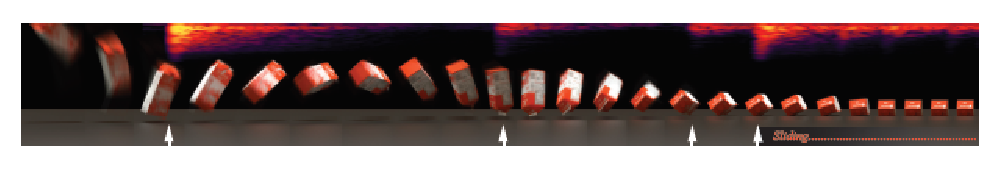
\includegraphics[width=15cm]{fig/chap2/IFA.eps}
%	\caption{落下アニメーションの自動生成結果}
%	\label{fig:IFA}
%\end{figure}
%
\indent
キャラクタの口の動きと音声を同期させる,リップシンクという技術がある.
キャラクタの口の動きに合わせて後から音声を録音するアフレコは,アニメーションに合わせて台詞を収録するため,口元と台詞の同期が比較的容易である.
一方,音声に合った口元のアニメーションを生成するには,口の形や動きを音声と1つずつ合わせる必要がある.
また,映画の吹替え版では,役者の口と声にズレが生じることに,違和感を感じることがある.
上述の課題を解消するため,リップシンクは,近年注目を集めている技術の1つである.\\
\indent
Breglerら\cite{Bregler},Ezzatら\cite{Ezzat}は,既存の動画に映っている対象人物の口元のみを,音声データに合わせて再構成することにより,リップシンクを図る手法を提案した.
Edwardsら\cite{JALI}は,台詞が収録されている音源および台詞が記載されているテキストファイルを入力すると,その台詞を話している口元のアニメーションを自動生成する手法を提案した.
本手法では,顎と唇だけを制御することにより,自然な口元のアニメーションを自動生成している.さらに,後から表情を編集することが可能となっているため,より自然な表情のアニメーションを実現できる.\\
%\begin{figure}[h]
%	\centering
%	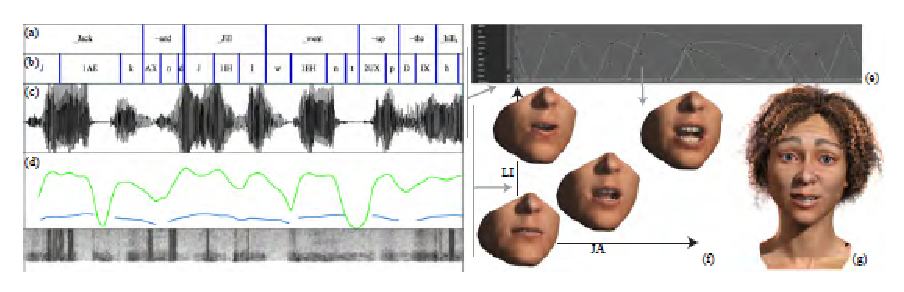
\includegraphics[width=15cm]{fig/chap2/JALI.eps}
%	\caption{口元アニメーションの自動生成}
%	\label{fig:JALI}
%\end{figure}
%
\indent
本研究の目的と同じように,音源から楽器を演奏するアニメーションを自動生成する研究も行われている.
Zhuら\cite{piano}は,MIDI音源からピアノを弾く指元のアニメーションを自動生成する手法を提案した.
ピアノのような鍵盤楽器は,指と音が一対一で対応していないため,フレーズにより指使いを変える必要がある.
ある指が他の指の上や下を通るような指使いのときは,指同士が衝突しないように考慮する必要もある.
彼らの手法では,これらの課題を解消することが可能である.\\
\indent
Yinら\cite{violin}は,wave音源からバイオリンを弾く手のアニメーションを自動生成する手法を提案した.
彼らは弦を押さえる左手の指元のアニメーションだけでなく,その指の動きが不自然に見えないような手首や腕の動きも再現している.
加えて,弓を持つ右手の動きも自動生成している.
Kimら\cite{violin2}も同様に,バイオリンを引く手のアニメーションを自動生成する手法を提案した.\\
\indent
ElKouraら\cite{ElKoura}は,ギターを弾く左手のアニメーションを自動生成する手法を提案した.
彼らの研究はギターの弾き方の指導を目的としており,アニメーションは音源から自動生成するのではなく,指を置く位置を入力することで生成される.\\
%\begin{figure}[h]
%	\centering
%	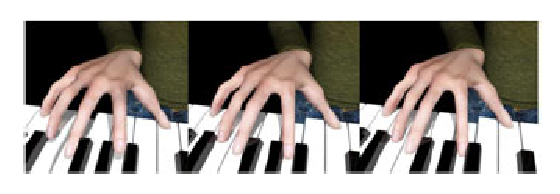
\includegraphics[width=15cm]{fig/chap2/piano.eps}
%	\caption{ピアノを弾く手元のアニメーションの自動生成}
%	\label{fig:piano}
%\end{figure}
%
\indent
上述の研究の他にも,音源に合った表情を自動生成する研究\cite{facial}\cite{DiPaola}\cite{morishima}や,音源に合ったダンスアニメーションを自動生成する研究\cite{dance2}\cite{dance1}など,さまざまなジャンルに着目した研究が存在する.

\section{アニメーションから音を生成する研究}\label{sec:generate_sound}
音とアニメーションを同期させることを目的として,物理シミュレーションの結果を音に反映させる研究分野が存在する.
以下では,その分野に関連した研究を紹介する.\\
%
\subsection{サウンドレンダリング}
サウンドレンダリングとは,物理アニメーションを生成すると同時に音を生成することにより,双方を同期させることを目的とする研究分野である.
この分野は,1992年に発表されたTakalaらの論文\cite{sound}が発端となっている.
彼らは,音の実態が光と同じ波動であること,音が物体の動きに依存することに着目して,音をレンダリングにより自動生成する手法を提案した.
%CG-ARTSの教育リポート,『音を描き出す夢の実現』\cite{CG-ARTS}によると,本分野は1990年代前半に登場し,未だ実験的にとどまっている分野となっている.
2009年には1つのシミュレーションパイプラインのなかで,CGアニメーションと,それに呼応した音を同時に生成するアルゴリズム\cite{james1}がZhengにより考案された.
本アルゴリズムでは,自然な流水音が,流水アニメーションから自動生成される.
また,自動生成された流水音は,アニメーションと完全に同期している.
%\begin{figure}[h]
%	\centering
%	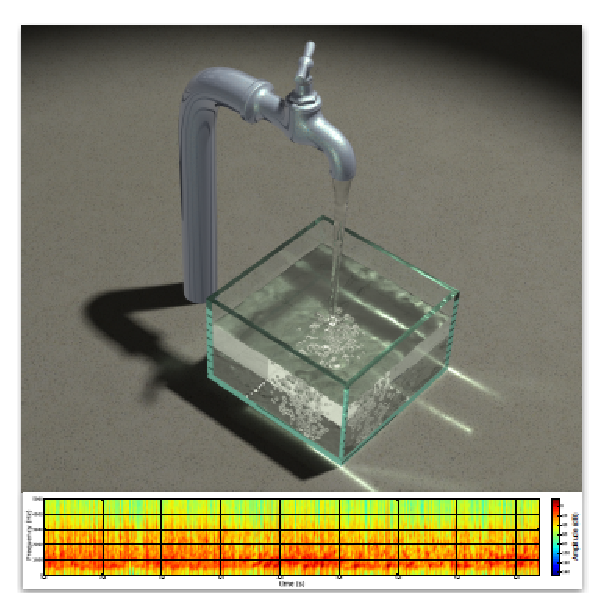
\includegraphics[width=15cm]{fig/chap2/james1.eps}
%	\caption{水のアニメーションと音の同時生成結果}
%	\label{fig:james1}
%\end{figure}
%
翌年には,同氏らにより破壊音を自動生成するアルゴリズム\cite{james2}が発表された.
本アルゴリズムでは,さまざまな剛体の破壊音だけでなく,その衝撃が間接的におよぼす影響も考慮されている.
そのため,複数の物体がぶつかり合い,破壊し合うようなアニメーションでも,そのアニメーションに同期する音が,忠実に再現された.
%\begin{figure}[h]
%	\centering
%	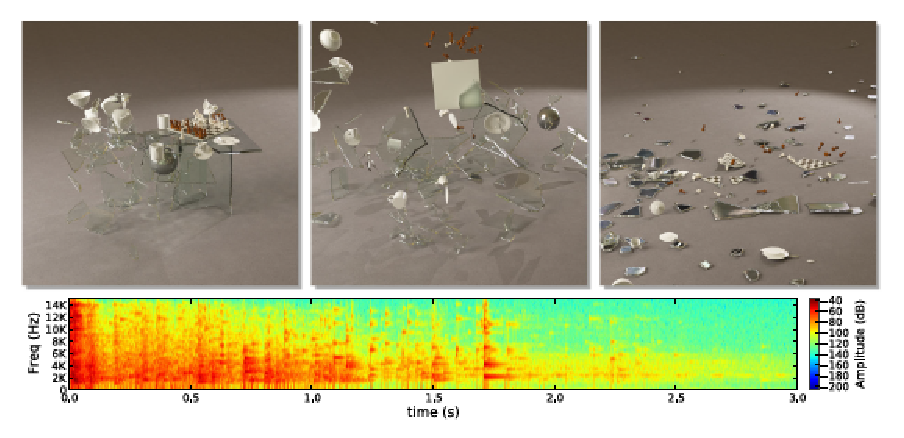
\includegraphics[width=14cm]{fig/chap2/james2.eps}
%	\caption{複数の剛体がぶつかり破壊される様子}
%	\label{fig:james2}
%\end{figure}
%
\subsection{プロシージャルオーディオ}
プロシージャルオーディオとは,作り置きした音を必要なタイミングで再生するのではなく,その都度プログラムで作り出す技術である.
ゲームソフトを開発している株式会社スクウェア・エニックスは本技術を研究しており,2014年のCEDECにて詳細\cite{SQUARE}を発表した.\\
\indent
ゲームでは,プレイヤの操作に応じてシステム内で効果音が選択され,再生される.
それらの音は,一般的には事前に作成し,システムに記憶させておく.
しかし,ゲームは使用可能な記憶領域が限られているため,可能な限りメモリを節約したい.
そのようなときに,本技術はひじょうに役立つ.
また,物体の挙動に合わせて音を自動生成するため,自然な効果音を再現することができる.

\section{音とアニメーションを同期させる研究} \label{sec:synchronization}
音やアニメーションを,もう一方から自動生成する研究だけでなく,既に生成されている双方を編集することにより同期させる研究も存在する.
Leeら\cite{Lee}は,MIDI音源およびキャラクタのモーションデータを入力とし,双方を最小限編集することにより,MIDI音源と同期したキャラクタのダンスアニメーションを生成する手法を提案した.\\
%\begin{figure}[h]
%	\centering
%	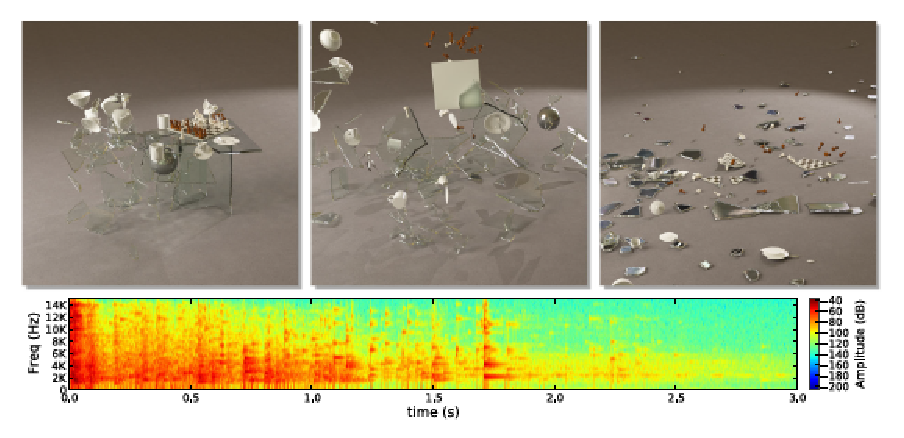
\includegraphics[width=15cm]{fig/chap2/james2.eps}
%	\caption{ダンスアニメーションと音を同期}
%	\label{fig:lee}
%\end{figure}
\indent
この研究分野は,複数のカットを組み合わせて作成するモンタージュの作成にも応用されている.
Liaoら\cite{Liao}は,BGMとなる音源および複数のビデオクリップを入力することにより,BGMに合ったモンタージュを作成する手法を提案した.

\section{ユーザの表情をキャラクタに反映する研究} \label{sec:animoji}
2017年秋に発売されたiPhoneXには,アニ文字という機能がある.
この機能は,カメラで認識したユーザの表情を,デバイス内のキャラクタに反映することができる.
このように,ユーザの表情をカメラで認識することにより,キャラクタのフェイシャルアニメーションを自動生成することを目的とした研究が存在する.\\
\indent
Weiseら\cite{Weise}は,カメラを用いてユーザの顔のモーションをキャプチャすることにより,顔のモーションデータを取得し,
それを仮想世界のキャラクタの顔に反映する手法を提案した.
顔のモーションキャプチャにはマーカーが必要がない.
また,キャプチャ中に手などにより顔が遮られた場合は,自動的に補正される仕組みとなっている.
なお,反映されるキャラクタは,人型のキャラクタのみである.
この研究を行っていたメンバーの1人であるPauly\cite{Pauly}は,2年後に,トラッキングの際に深さを考慮することにより,トラッキングの質を向上させた.
そのことにより,しわなど皮膚の細かい情報もキャラクタに反映されるようになった.\\
\indent
同年にXuら\cite{Xu}は,顔のモーションデータを人型ではないキャラクタの顔に反映する手法を提案した.

\section{吹奏楽に関連した研究} \label{sec:marching}
マーチングとは,演奏者が演奏しながら定められた経路に従って歩くことにより隊形を作る,吹奏楽の演奏形態である.
本論文の筆者は,マーチングを行う1名の演奏者の軌跡を可視化することにより,その演奏者が歩くべき経路と実際の経路の誤差を表示するシステム(\figref{fig:marching})を提案した.
軌跡の可視化には,物体追跡アルゴリズムの1つであるLucas Kanade法\cite{Lucas}が用いられている.
本システムにより,演奏者は自身の歩行の改善点を知ることができ,その結果マーチングの隊形の完成度を高めることが期待できる.
\begin{figure}[H]
	\centering
	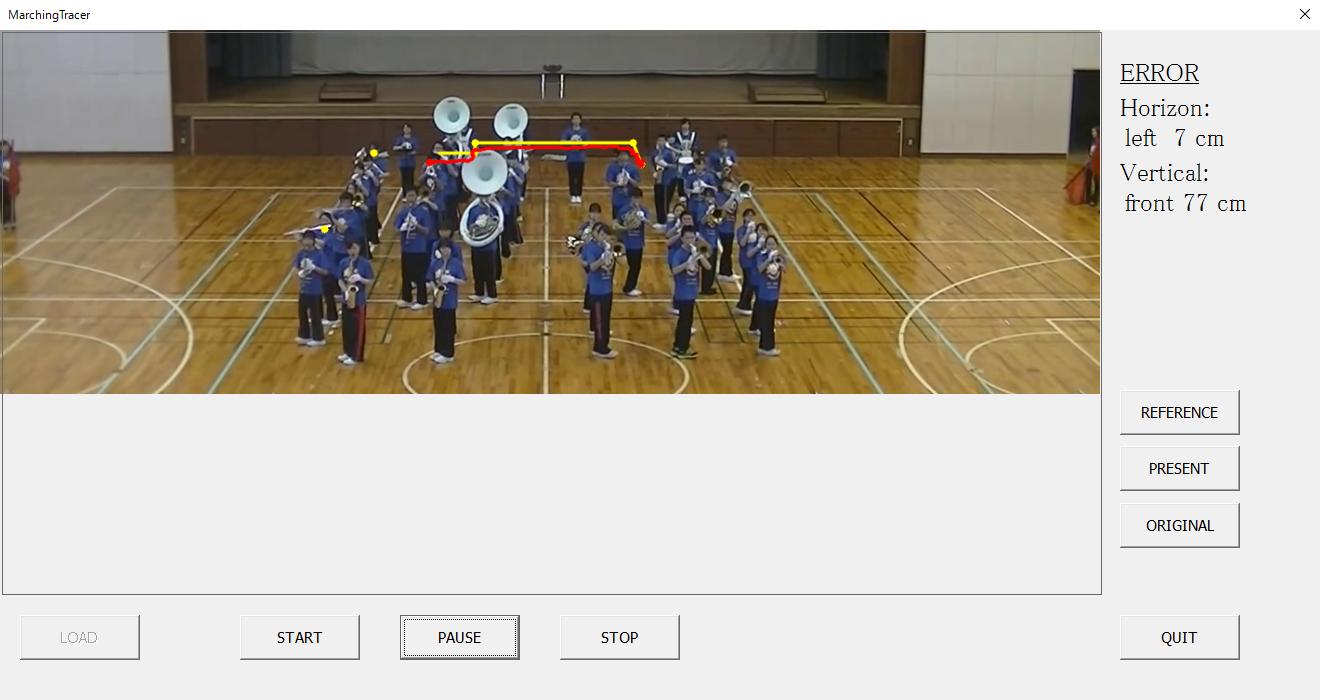
\includegraphics[width=14cm]{fig/chap2/marching.eps}
	\caption{マーチングを行う演奏者の軌跡および誤差の表示例}
	\label{fig:marching}
\end{figure}
なお,この研究の成果は,NICOGRAPH2016においてポスター\cite{nicograph}にて発表した.
そして,一連の研究をまとめた成果が,画像電子学会誌のVol.47\cite{iieej}に掲載される予定である.

\section{本研究の新規性}\label{sec:compere}
アニメーションと音の同期や,吹奏楽をテーマとした研究は多く存在する.
しかし,管楽器を演奏するキャラクタと音の同期に注目した研究は存在しない.
また,\secref{sec:generate_animation}で挙げた,ピアノやバイオリンを演奏するアニメーションの自動生成を目的とした研究では,複数名での演奏は考慮されていない.
したがって本研究の新規性は,管楽器を複数名で演奏するアニメーションを,音から自動生成するという点である.
さらに,本論文ではトランペット奏者およびトロンボーン奏者に適用した例だけを示すが,音と指使いの対応表を用意することにより,すべての管楽器の演奏アニメーションが入力音源から自動生成できる.
このように,あらゆる楽器への対応が可能である点も,新規性があるといえる.